\section{Method}
\label{sec:method}

\subsection{Problem Formulation}

A test video $V$ has $N$ frames recorded at $f$ frames per second. The task is to produce a tuple $(t^{*}, c_x^{*}, c_y^{*}, k^{*})$: $t^{*}$ is the accident time in seconds, $(c_x^{*}, c_y^{*}) \in [0, 1]^{2}$ are normalized image coordinates of the point of impact, and $k^{*} \in \mathcal{K}$ is the collision type. The label space is $\mathcal{K} = \{\texttt{head-on}, \texttt{rear-end}, \texttt{sideswipe}, \texttt{single}, \texttt{t-bone}\}$.

We split the problem into three parts. Time and location predictions rely on classical signal processing; type classification relies on a pre-trained vision-language model.

\subsection{Temporal Peak Detection}

Collisions produce sudden intensity changes between consecutive frames. We exploit this observation by building a one-dimensional signal from per-frame brightness differences and then looking for statistical outliers in that signal.

Let $I_t \in \mathbb{R}^{H \times W}$ be the grayscale frame at index $t$, resized to $H = 180$, $W = 320$ for speed. We compute the mean absolute difference between adjacent frames:
\begin{equation}
    d_t = \frac{1}{HW} \sum_{u=1}^{H} \sum_{v=1}^{W} \big| I_{t+1}(u,v) - I_t(u,v) \big|
    \label{eq:framediff}
\end{equation}
for $t = 1, \ldots, N{-}1$. This series contains both collision signals and background noise from camera shake and ordinary traffic. A centered rolling mean with window $w = 5$ suppresses the short-lived noise:
\begin{equation}
    \bar{d}_t = \frac{1}{|W_t|} \sum_{s \in W_t} d_s
    \label{eq:smooth}
\end{equation}
where $W_t = \{s : |s - t| \leq \lfloor w/2 \rfloor\}$. We normalize the smoothed values into z-scores using the series-wide mean $\mu$ and standard deviation $\sigma$:
\begin{equation}
    z_t = \frac{\bar{d}_t - \mu}{\sigma + \varepsilon}
    \label{eq:zscore}
\end{equation}
with $\varepsilon = 10^{-8}$ to avoid division by zero. Any frame whose $z_t$ exceeds a threshold $\tau$ is treated as an anomaly candidate. Among all candidates, we select the one with the strongest anomaly score:
\begin{equation}
    t^{*}_{\text{frame}} =
    \begin{cases}
        \arg\max_{t :\, z_t > \tau}\, z_t & \exists\, t \text{ s.t. } z_t > \tau \\
        \arg\max_t\, z_t & \text{otherwise}
    \end{cases}
    \label{eq:peak}
\end{equation}
with $\tau = 1.5$. Taking the highest-scoring candidate among threshold-crossers favors the most prominent motion event. When no frame crosses the threshold, we fall back to the global maximum. Time in seconds is $t^{*} = t^{*}_{\text{frame}} / f$.

Figure~\ref{fig:temporal_signal} shows the raw frame-difference series and its z-score transform for a synthetic head-on collision. The raw signal (top panel) contains a mixture of gradual intensity drift from vehicle motion and a sharp transient near the collision moment. After smoothing and normalization (bottom panel), the collision event stands out as a distinct peak while background variation stays below the detection threshold.

\begin{figure}[t]
    \centering
    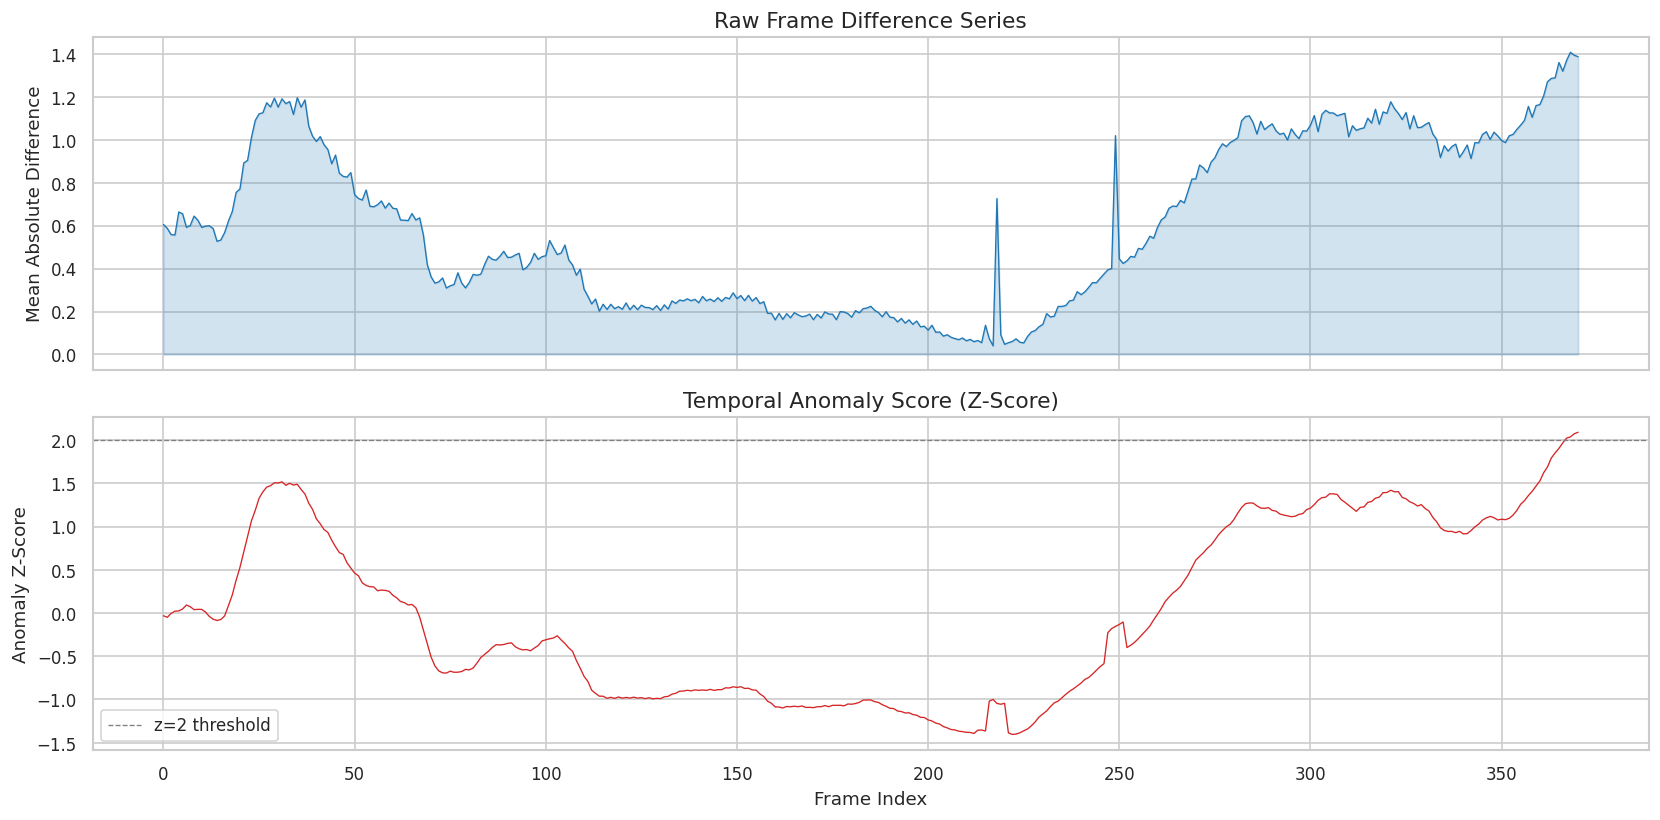
\includegraphics[width=\linewidth]{fig/frame_diff_zscore.png}
    \caption{Temporal localization on a synthetic CARLA video. Top: mean absolute frame difference $d_t$ across all frames. Bottom: z-score anomaly series $z_t$ after rolling-mean smoothing. The dashed line marks the detection threshold.}
    \label{fig:temporal_signal}
\end{figure}

\subsection{Spatial Impact Localization}

A collision concentrates high-magnitude motion in a small region of the image. We identify that region by accumulating dense optical flow over a short window and then computing the weighted centroid of the resulting magnitude map.

When the predicted accident time $t^{*}$ is available from the temporal module, we center a 30-frame window on the corresponding frame index; otherwise, we fall back to starting at frame $\lfloor N/3 \rfloor$. For each pair of consecutive frames within this window, we run the Farneback dense optical flow algorithm~\cite{farneback2003two} at $320 \times 180$ resolution. Farneback estimates per-pixel displacement using quadratic polynomial expansions and a multi-scale Gaussian pyramid. We set pyramid scale to $0.5$, three levels, window size $15$, three iterations, and polynomial parameters $n = 5$, $\sigma_p = 1.2$.

Let $\mathbf{f}_t(u,v) = (f_x, f_y)$ be the flow vector at pixel $(u,v)$ between frames $t$ and $t{+}1$. We sum the displacement magnitudes:
\begin{equation}
    M(u,v) = \sum_{t} \sqrt{f_{x}^{\,2}(u,v,t) + f_{y}^{\,2}(u,v,t)}
    \label{eq:magmap}
\end{equation}
Before extracting the centroid, we apply a percentile threshold at the 90th percentile of $M$ and zero out all values below it. This suppresses diffuse background motion and retains only the high-magnitude cluster near the collision site. The impact location is the weighted centroid of the thresholded map, normalized to unit coordinates:
\begin{equation}
    c_x^{*} = \frac{1}{W}\,\frac{\sum_{u,v} v \cdot M(u,v)}{\sum_{u,v} M(u,v)}, \quad
    c_y^{*} = \frac{1}{H}\,\frac{\sum_{u,v} u \cdot M(u,v)}{\sum_{u,v} M(u,v)}
    \label{eq:centroid}
\end{equation}
If $\sum M < 10^{-6}$, we return the frame center $(0.5, 0.5)$. This centroid calculation is a special case of the image moment framework introduced by Hu~\cite{hu1962visual}, applied to flow magnitudes instead of pixel intensities.

Figure~\ref{fig:heatmap} shows the accumulation result on a synthetic video. The collision region concentrates most of the optical flow energy into a compact spatial cluster. After percentile thresholding, the weighted centroid falls within that cluster and provides a localized impact coordinate.

\begin{figure}[t]
    \centering
    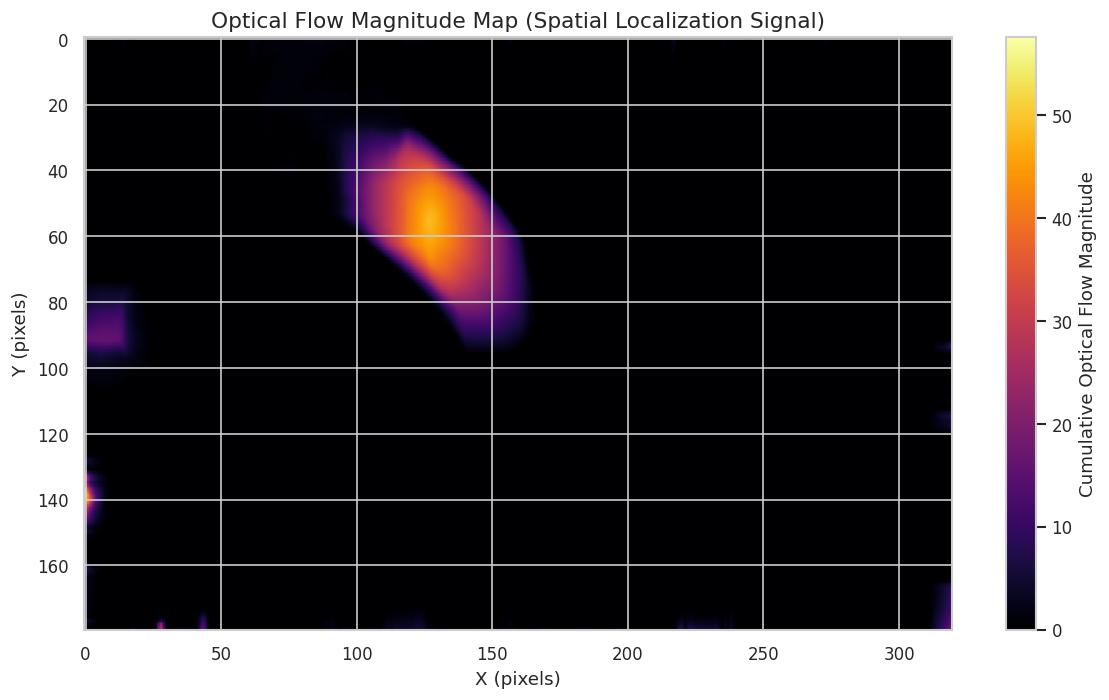
\includegraphics[width=\linewidth]{fig/heatmap.png}
    \caption{Cumulative Farneback optical flow magnitude $M(u,v)$ on a synthetic CARLA video after 90th-percentile thresholding. The bright region corresponds to the collision area; diffuse background motion is suppressed.}
    \label{fig:heatmap}
\end{figure}

\subsection{Collision Type Classification}

We assign a collision type using CLIP~\cite{radford2021learning}, which learns a joint embedding space for images and text by contrastive training on 400 million image-text pairs collected from the internet. At test time, CLIP compares an image embedding against text embeddings of candidate class names using cosine similarity, allowing classification without any task-specific training data.

For each type $k \in \mathcal{K}$, we write five natural language descriptions $\{p_k^1, \ldots, p_k^5\}$ that characterize the collision from a bystander perspective (Table~\ref{tab:prompts}). Using several prompts per class reduces the influence of any one particular wording, consistent with the prompt ensembling approach studied by Radford et al.~\cite{radford2021learning} and Zhou et al.~\cite{zhou2022learning}. Each prompt is encoded by the CLIP text encoder $\phi_{\text{text}}$, L2-normalized, and then averaged:
\begin{equation}
    \mathbf{t}_k = \frac{1}{5} \sum_{j=1}^{5} \frac{\phi_{\text{text}}(p_k^j)}{\|\phi_{\text{text}}(p_k^j)\|}
    \label{eq:textfeat}
\end{equation}
These vectors are computed once and cached before processing any video.

At inference time, we extract eight video frames centered on the predicted accident time $t^{*}$ and feed them into the CLIP visual encoder (ViT-B/32). Each embedding is L2-normalized, and we average the eight into a single representation:
\begin{equation}
    \mathbf{v} = \frac{1}{8} \sum_{i=1}^{8} \frac{\phi_{\text{img}}(I_{t_i})}{\|\phi_{\text{img}}(I_{t_i})\|}
    \label{eq:imgfeat}
\end{equation}
The predicted type is the class with highest similarity:
\begin{equation}
    k^{*} = \arg\max_{k \in \mathcal{K}} \; \mathbf{v} \cdot \mathbf{t}_k
    \label{eq:classify}
\end{equation}

\begin{table}[t]
\centering
\small
\caption{Prompt templates for collision type classification. Five prompts per class are averaged into one text embedding.}
\label{tab:prompts}
\begin{tabular}{@{}ll@{}}
\toprule
\textbf{Type} & \textbf{Example prompt} \\
\midrule
head-on   & ``two cars colliding head-on from opposite directions'' \\
rear-end  & ``a car colliding into the back of another car'' \\
sideswipe & ``two vehicles scraping alongside each other'' \\
single    & ``a single car crashing into a wall or obstacle'' \\
t-bone    & ``a car hitting the side of another car at an intersection'' \\
\bottomrule
\end{tabular}
\end{table}
